\noindent

\includegraphics[height=1.25cm]{images/pictograms/replication}
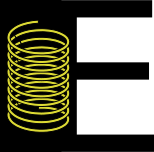
\includegraphics[height=1.25cm]{images/pictograms/elasticity}

\includegraphics[height=1.25cm]{images/pictograms/benchmark}
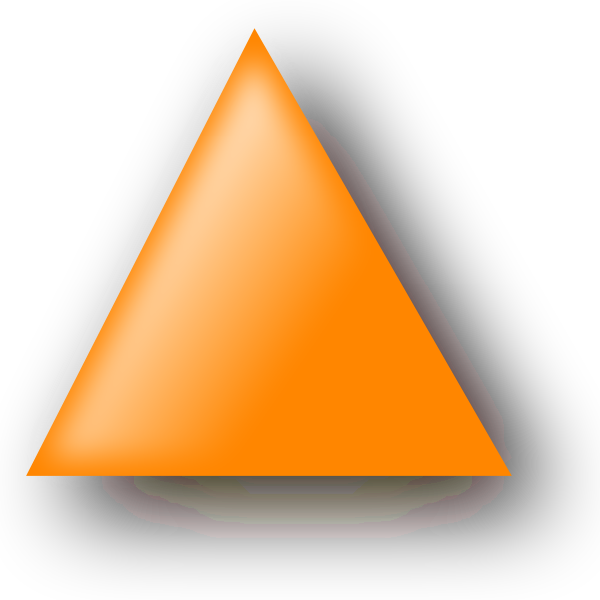
\includegraphics[height=1.25cm]{images/pictograms/triangle}

\includegraphics[height=1.25cm]{images/pictograms/FEM}

\includegraphics[height=1.25cm]{images/pictograms/paraview}

%%%%%%%%%%%%%%%%%%%%%%%%%%%%%%%%%%%%%%%%%%%%%%%%%%%%%%%%%%%%%%%%%%%%%%%%%%%%%%%%%%%%%%%%%%%%%%%%%%%

\begin{flushright} {\tiny {\color{gray} python\_codes/fieldstone\_179/text.tex}} \end{flushright}

\par\noindent\rule{\textwidth}{0.4pt}

\begin{center}
\inpython
{\small Code: \url{https://github.com/cedrict/fieldstone/tree/master/python_codes/fieldstone_179}}
\end{center}

\par\noindent\rule{\textwidth}{0.4pt}

Last revision: September 13th, 2025.

\par\noindent\rule{\textwidth}{0.4pt}

%%%%%%%%%%%%%%%%%%%%%%%%%%%%%%%%%%%%%%%%%%%%%%%%%%%%%%%%%%%%%%%%%%%%%%%%%%%%%%%%%%%%%%%%%%%%%%%%%%%

This \stone is inspired by \textcite{koko07} (2007) in which the author presents 
a clever way to build and assemble elemental matrices for a 2d $P_1$ elastic code.
The 'clever' way is presented in Section~\ref{MMM-ss:p1}.

%------------------------------------------------
\section*{The physical problem}

The domain $\Omega$ is described by the polygon
$(-1,-1), (0,-2), (2, 0), (0, 2), (-1,+1), (0, 0)$.

The exact solution is known in polar coordinates $(r,\theta)$:
\begin{eqnarray}
u_r(r,\theta)
&=&\frac{1}{2\mu} r^\alpha 
[(c_2 - \alpha - 1)c_1 \cos((\alpha - 1)\theta) 
- (\alpha + 1) \cos((\alpha + 1)\theta)] \nn\\
u_\theta(r,\theta)&=& 
\frac{1}{2\mu}
[(\alpha + 1) \sin((\alpha + 1)\theta) 
+ (c_2 + \alpha - 1)c_1 \sin((\alpha - 1)\theta)]
\end{eqnarray}
The exponent $\alpha$ is the solution of the equation
\[
\alpha \sin(2\omega) + \sin(2\omega \alpha ) = 0
\]
with $\omega=3\pi/4$ and
\[
c_1 = -\frac{\cos((\alpha+1)\omega)}{\cos((\alpha-1)\omega)}
\qquad
\qquad
c_2 = 2 \frac{\lambda + 2\mu}{\lambda+\mu}
\]

The displacement field is solution of the momentum equation 
with no body force ($\vec{f} = \vec{0}$) and $u_D = (u_r , u_\theta )$ on 
$\Gamma = \Gamma_D$. Numerical
experiments are carried out with Young's modulus $E = 100000$ 
and Poisson’s coefficient $\nu$ = 0.3. The magnitude of
the gradient $|\vec\nabla \vec{u}|$ of the exact solution 
has a singularity at the re-entrant corner $(0,0)$. This singularity,
despite being very local, is a significant source of error.

%------------------------------------------------
\section*{Implementation}

I have implemented the FEM matrix \& rhs building process as I 
usuallly do (e.g. \stone~58), i.e. using Gauss quadrature and
coined it \lstinline{method=0}.
I also implemented the clever way of \textcite{koko07} (2007)
as explained in Section~\ref{MMM-ss:p1}. It bypasses Gauss quadrature
altogether and allows to build elemental matrices and rhs directly.
This is coined \lstinline{method=1}.
Note that in both cases the imposition of boundary conditions on the 
elemental matrices and their assembly is similar\footnote{Note 
that a faster assembly methods s here used as explained in \stone~176.} 
However because of how the elemental matrix is build in the second case
(4 blocks of size $3\times 3$: $\K_{xx}$, $\K_{yy}$, $\K_{xy}=\K_{yx}^T$)
it makes more sense to organise the global solution vector 
\[
\vec{\cal U}^T=(u_1,u_2, ...u_N,v_1,v_2,... v_N)
\]
This has consequences for the structure of the boundary conditions arrays, 
the boundary conditions imposition, the assembly and the recovery of 
the vectors $\vec{u}=(u_1,u_2,...u_N)$ and $\vec{v}=(v_1,v_2,...v_N)$. 
For example:
\begin{lstlisting}
if method==0:
   for i in range(0,nn_V):
       if on_boundary[i]: 
          ui,vi=displ_th(x_V[i],y_V[i])
          bc_fix_V[i*ndof_V+0] = True ; bc_val_V[i*ndof_V+0] = ui
          bc_fix_V[i*ndof_V+1] = True ; bc_val_V[i*ndof_V+1] = vi

else:
   for i in range(0,nn_V):
       if on_boundary[i]: 
          ui,vi=displ_th(x_V[i],y_V[i])
          bc_fix_V[i     ]=True ; bc_val_V[i     ]=ui
          bc_fix_V[i+nn_V]=True ; bc_val_V[i+nn_V]=vi
\end{lstlisting}

Remark: The author resorts to penalization to impose Dirichlet 
boundary conditions but details how to carry out Neumann boundary conditions.

Meshing is carried out as explained in \stone~131 and leads to such a mesh:
\begin{center}
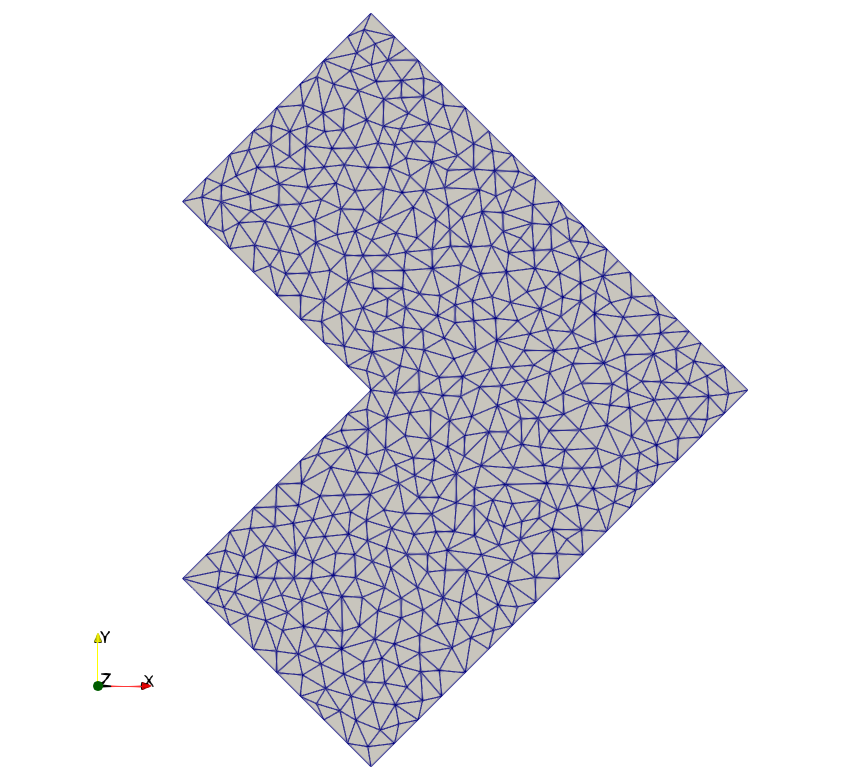
\includegraphics[width=8cm]{python_codes/fieldstone_179/RESULTS/mesh}
\end{center}

\newpage
%------------------------------------------------
\section*{Results}

After having verified that results are identical when either 
of the methods is used, we can visualise results:

\begin{center}
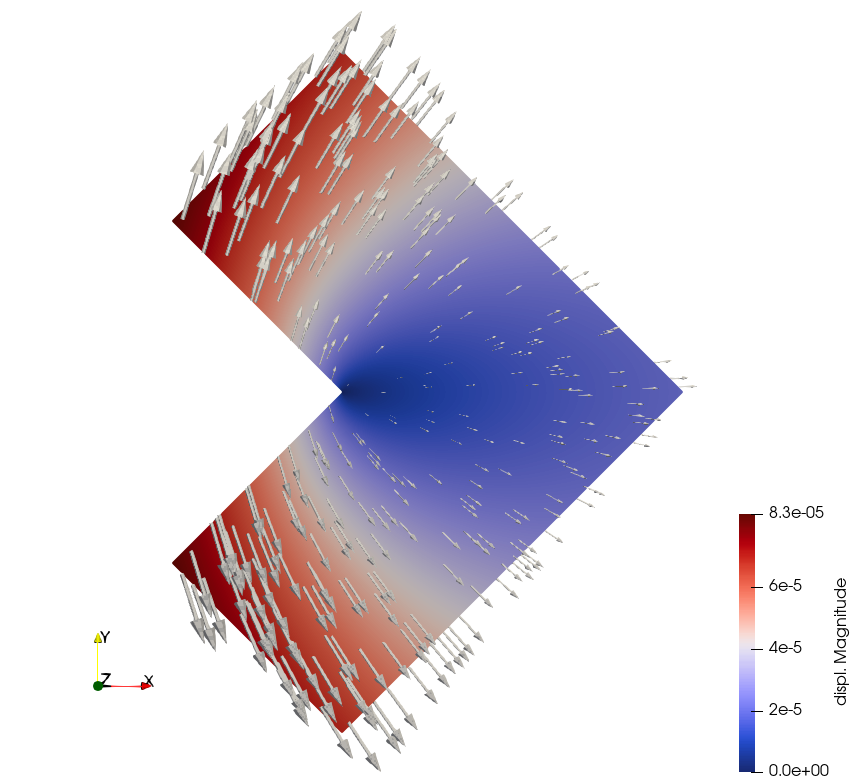
\includegraphics[width=7cm]{python_codes/fieldstone_179/RESULTS/disp}
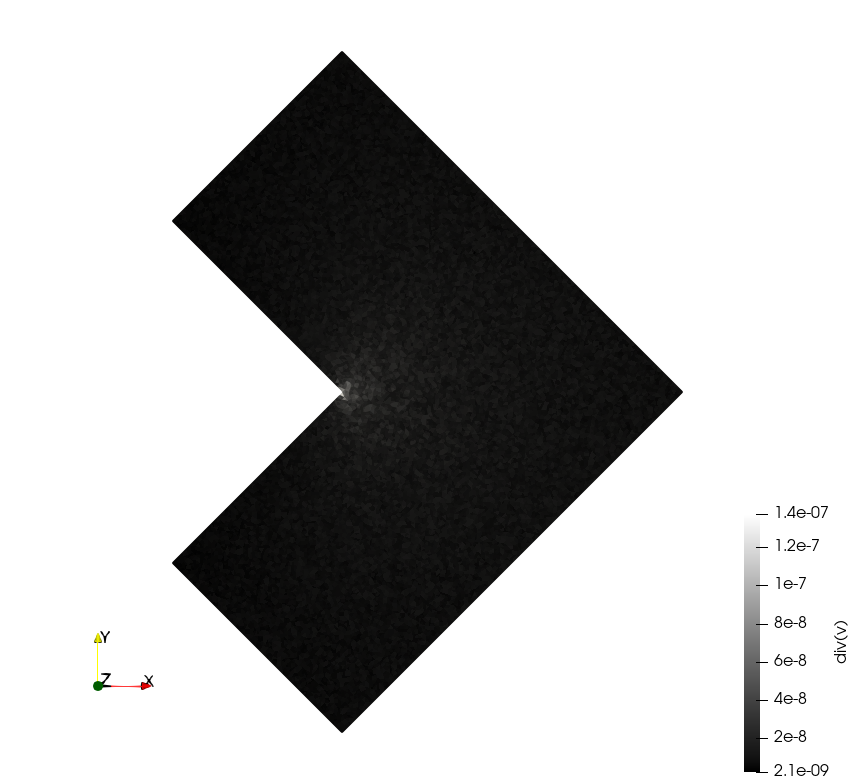
\includegraphics[width=7cm]{python_codes/fieldstone_179/RESULTS/divv}\\
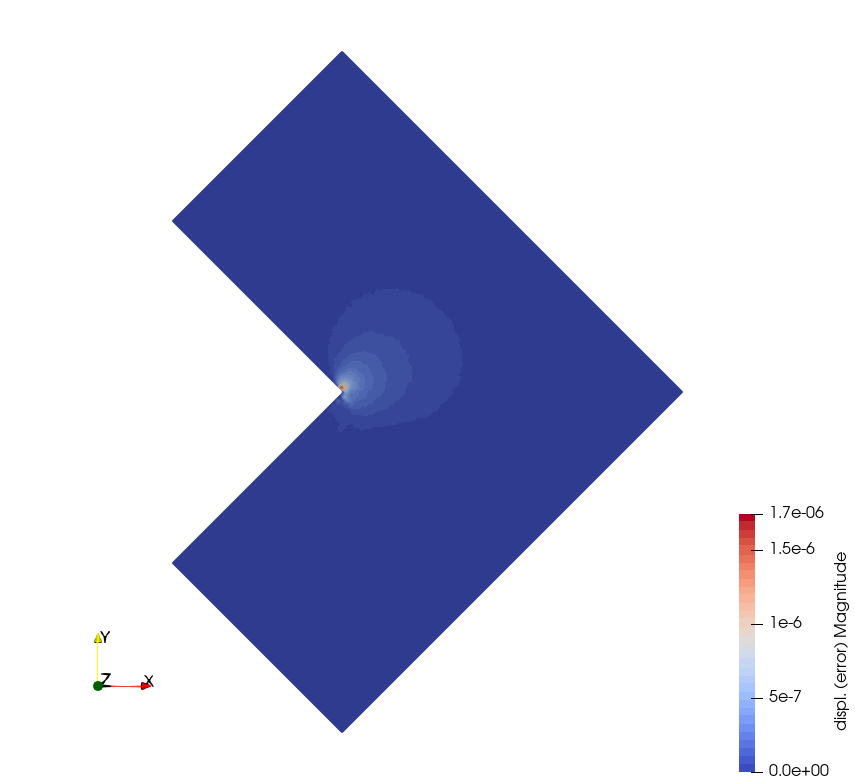
\includegraphics[width=7cm]{python_codes/fieldstone_179/RESULTS/error}
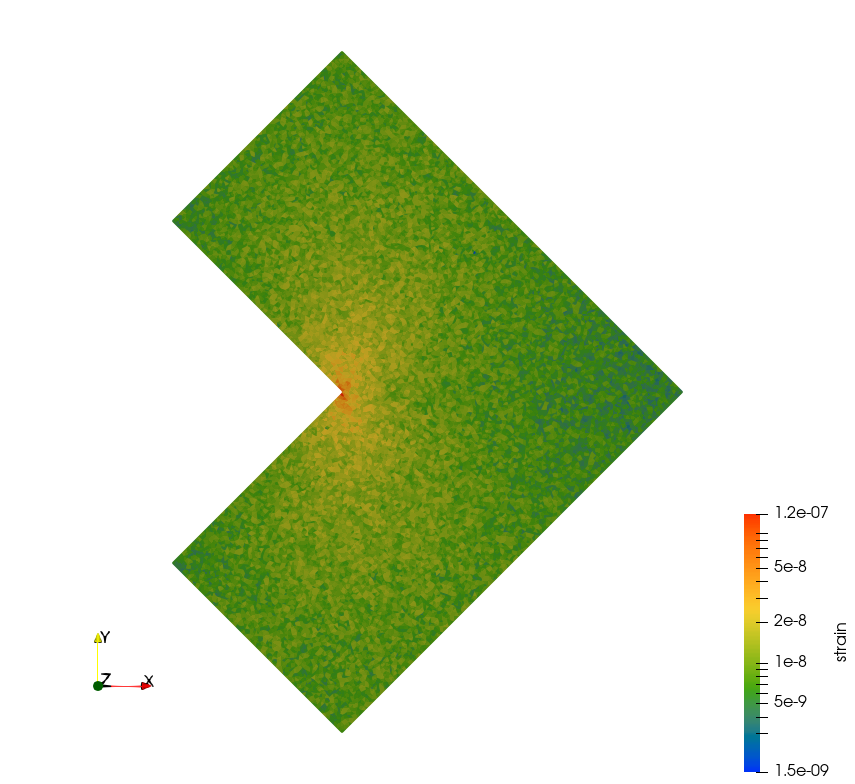
\includegraphics[width=7cm]{python_codes/fieldstone_179/RESULTS/strain}
\end{center}

By means of the {\tt script\_errors} bash script we can run models 
of increasing resolution and measure the matrix building time and the 
solve time.
\begin{center}
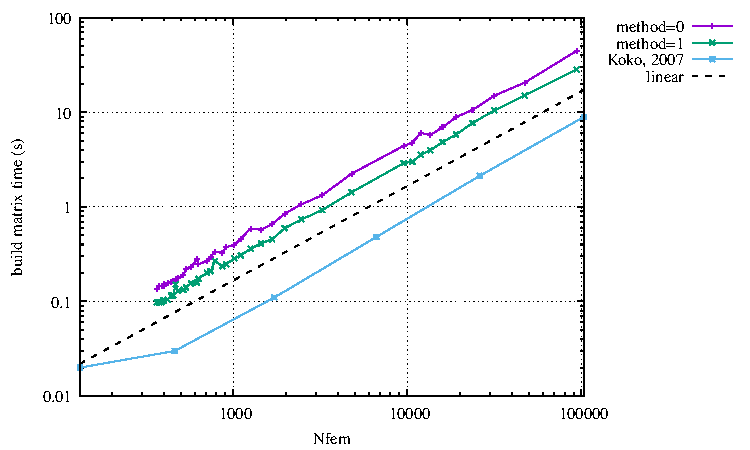
\includegraphics[width=8cm]{python_codes/fieldstone_179/RESULTS/build.pdf}
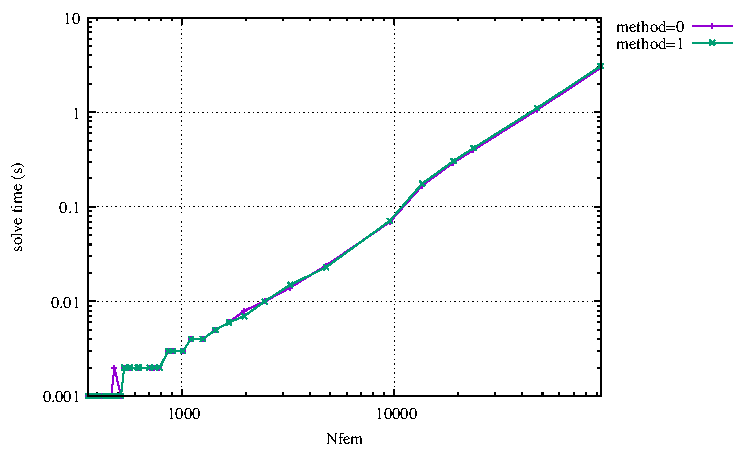
\includegraphics[width=8cm]{python_codes/fieldstone_179/RESULTS/solve.pdf}\\
{\captionfont Left: matrix building time (Koko's MATLAB timings are included);
Right: solve time.}
\end{center}

Because the build time also encompasses the boundary conditions and 
assembly, I also only measure the time need to build the elemental matrices:
\begin{center}
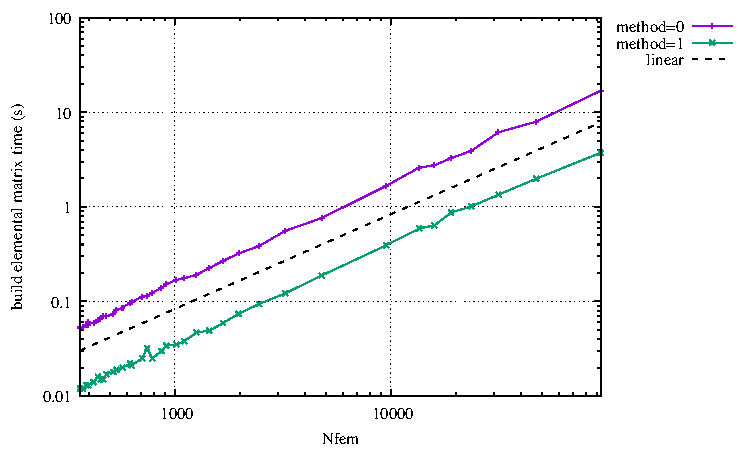
\includegraphics[width=10cm]{python_codes/fieldstone_179/RESULTS/Ael.pdf}
\end{center}
In this case the conclusion is clear: Koko's method is about 3 times faster.

Because of the structure of $\vec{\cal U}$ the assembled FEM matrices 
non-zero structure look very different:
\begin{center}
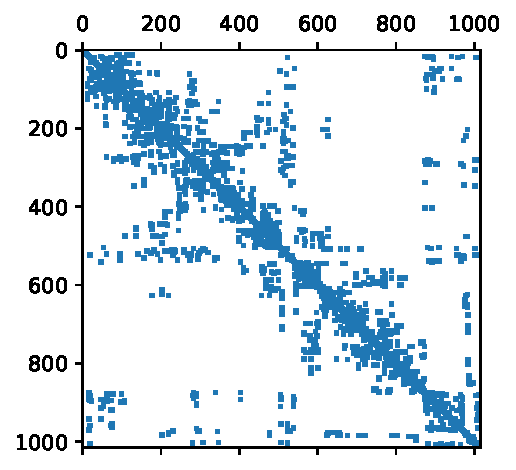
\includegraphics[width=8cm]{python_codes/fieldstone_179/RESULTS/matrix0.pdf}
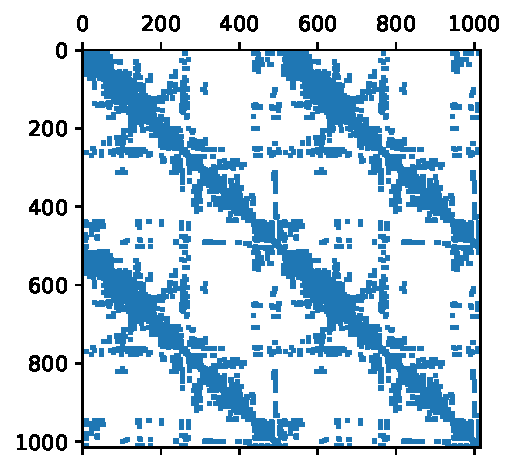
\includegraphics[width=8cm]{python_codes/fieldstone_179/RESULTS/matrix1.pdf}\\
{\captionfont Left: method=0; Right: method=1.}
\end{center}
Despite this difference in structure we find that the solve time is identical
in both cases.

Finally we can look at the discretisation error (as a function of 
the total number of dofs for commodity):
\begin{center}
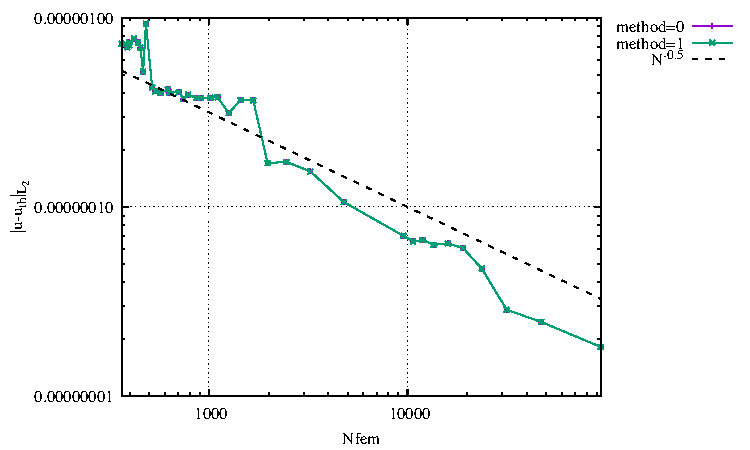
\includegraphics[width=10cm]{python_codes/fieldstone_179/RESULTS/erru.pdf}
\end{center}


\includegraphics[width=3cm]{images/conclusion} 
This is an interesting avenue, as long as material properties can 
be assumed to be constant inside each element.



